\documentclass{article}

\usepackage{booktabs}
\usepackage{tabularx}
\usepackage{graphicx}
\usepackage{float}

\input{../../Comments}
\input{../../Common}

\title{Usability Testing\\\progname}

\author{\authname}

\date{}

\begin{document}

\begin{table}[hp]
\caption{Revision History} \label{TblRevisionHistory}
\begin{tabularx}{\textwidth}{llX}
\toprule
\textbf{Date} & \textbf{Developer(s)} & \textbf{Change}\\
\midrule
April 2, 2025 & NFI & Initial setup of document.\\
\bottomrule
\end{tabularx}
\end{table}

\newpage

\maketitle

~\newpage

\pagenumbering{roman}

\tableofcontents

\listoffigures

~\newpage

\section{Introduction}
    \subsection{Purpose}
    This document outlines the usability testing plan for \progname. The goals of the
    testing is to evaluate user interactions with the system, identify issues the user
    may have with a part of the system's functionality, and quantify the results into
    a measureable format that can be analyzed.

    The analysis of results will allow developers of the system to improve upon
    the system iteratively as user feedback is continuously provided from the usability
    testing. The system will be improved upon by implementing suggestions made by
    testers, the supervisor, and other stakeholders providing feedback.
    
    \subsection{Scope}
    The usability testing focuses on the core features of the system, including
    scheduling, user navigation, ease of use, account creation, and rescheduling.

\section{Testing Goals}
    \begin{itemize}
        \item Assess ease of use, accessibility, and navigation within the platform.
        \item Identify pain points in the scheduling, rescheduling, and account
        management process.
        \item Ensure satisfactory system performance.
        \item Gather feedback for future improvements.
    \end{itemize}

\section{Testing Conducted}
    \subsection{Participants}
    \begin{itemize}
        \item Commissioners
        \item New users
        \item Experienced users
        \item Technical users
        \item Non-technical users
    \end{itemize}
    
    \subsection{Procedure}
    \begin{enumerate}
        \item Start the tester on the home page without being signed in to a
        registered account.
        \item Request the tester to navigate towards the account registration process
        and register their own account, can be either a player or team account.
        \begin{itemize}
            \item If the tester is unsure how to register an account, record what
            issue they are experiencing and assist them in the registration process
            by guiding them to the next step. For example, if they are unsure of where
            to register an account, direct them to the register page and allow them to
            continue the registration process on their own, unless they require more
            assistance.
        \end{itemize}
        \item Once completed, sign the tester into a preset team account.
        \item From the account page, as a team account, ask the tester to submit
        a reschedule request to another team.
        \begin{itemize}
            \item If the tester is unsure how to submit a reschedule request, record what
            issue they are experiencing and assist them in submitting a reschedule request
            by guiding them to the next step. For example, if they are unsure of where
            to start a reschedule request, direct them to the rescheduler screen and allow them to
            continue the rescheduling process on their own, unless they require more
            assistance.
        \end{itemize}
        \item Once completed, sign the tester into the team account they had submitted a
        reschedule request towards.
        \item From the account page, as the incoming reschedule request team account,
        ask the tester to accept the incoming reschedule request from the team they
        had just submitted the reschedule request from.
        \begin{itemize}
            \item If the tester is unsure how to accept a reschedule request, record what
            issue they are experiencing and assist them in accepting a reschedule request
            by guiding them to the next step. For example, if they are unsure of where
            to accept the reschedule request, direct them to the manage reschedule request page
            and allow them to continue the acceptance process on their own, unless they require more
            assistance.
        \end{itemize}
        \item Once completed, ask the tester to navigate to the scheduler screen to
        view the rescheduled game.
        \item Provide the usability survey to the tester to fill out.
    \end{enumerate}

\section{Usability Survey}
    A Microsoft Form will be provided to testers of the system to validate specific
    system tests outlined in the VnV plan. Answers for each question will range from either a
    rating between 1 (Strongly Disagree) to 5 (Strongly Agree), 1 (Very Difficult) to 5 (Very Easy), or
    1 (No, the system was difficult to use due to accessibility issues) to 3 (Yes, the system was accessible).
    A satisfactory result for each question should be a 3 (Neutral/Yes, the system was accessible) or above.
    Additionally, the team should address any issues the user has with the system, which will be received
    from optional questions located below each multiple choice question of the survey.
    \\\\Questions in the Microsoft Form can be accessed at the following link:\\

    \href{https://forms.office.com/Pages/ResponsePage.aspx?id=B2M3RCm0rUKMJSjNSW9HcodvkeIlB8lOjrmyIWuVT7dUQ0hBNFRVTjFHWVhITDIzSklZRDRYTVZRMi4u}{Sandlot Usability Survey}

\section{Results and Analysis}
    The usability testing of the Sandlot website revealed overall positive user
    experiences, with high ratings for readability, navigation, registration,
    and login processes.
    
    Testers found the website's text and images clear and
    well-formatted, and the registration system provided appropriate feedback,
    though additional security measures like two-factor authentication and
    password strength checks could enhance protection.
    
    Navigation was intuitive and login security was robust,
    but contextual help and tooltips could improve user guidance.
    \begin{itemize}
        \item Tooltips and contextual help were added on various pages. For
        example, a tooltip was added to provide users the proper formatting of
        a team username as well as password visibility icons that could be turned
        on and off, if users wanted to view the passwords they were typing.
    \end{itemize}

    \begin{figure}[H]
    \centering
    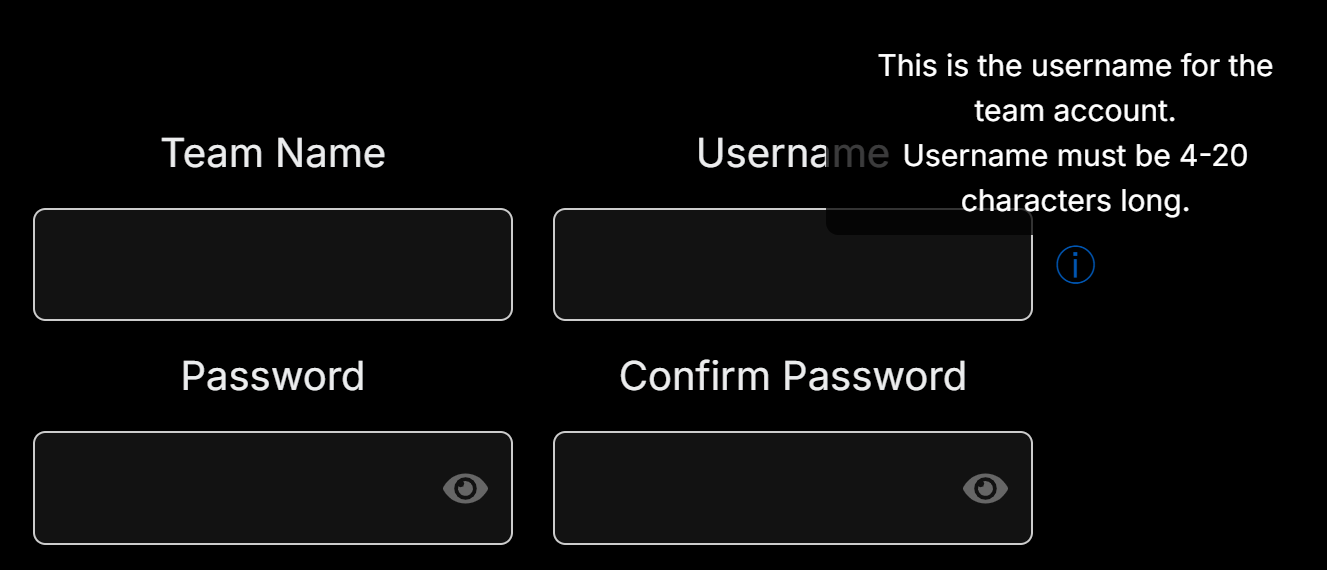
\includegraphics[scale=0.6]{tooltip_password_visibility.png}
    \caption{User Guidance Improvement}
    \label{guide}
    \end{figure}
    
    General access
    to the schedule and standings was seamless, but minor delays in page loading
    were noted. Furthermore, the reschedule request process
    needed refinement to ensure clearer feedback on user actions.

    \begin{itemize}
        \item The rescheduling interface experienced additions in color coding and
        a legend to identify what each color indicated in the reschedule process.
        This suggestion was crucial to implement to ensure a users' understanding
        and limit their confusion in an integral function of the system.
    \end{itemize}

    \begin{figure}[H]
    \centering
    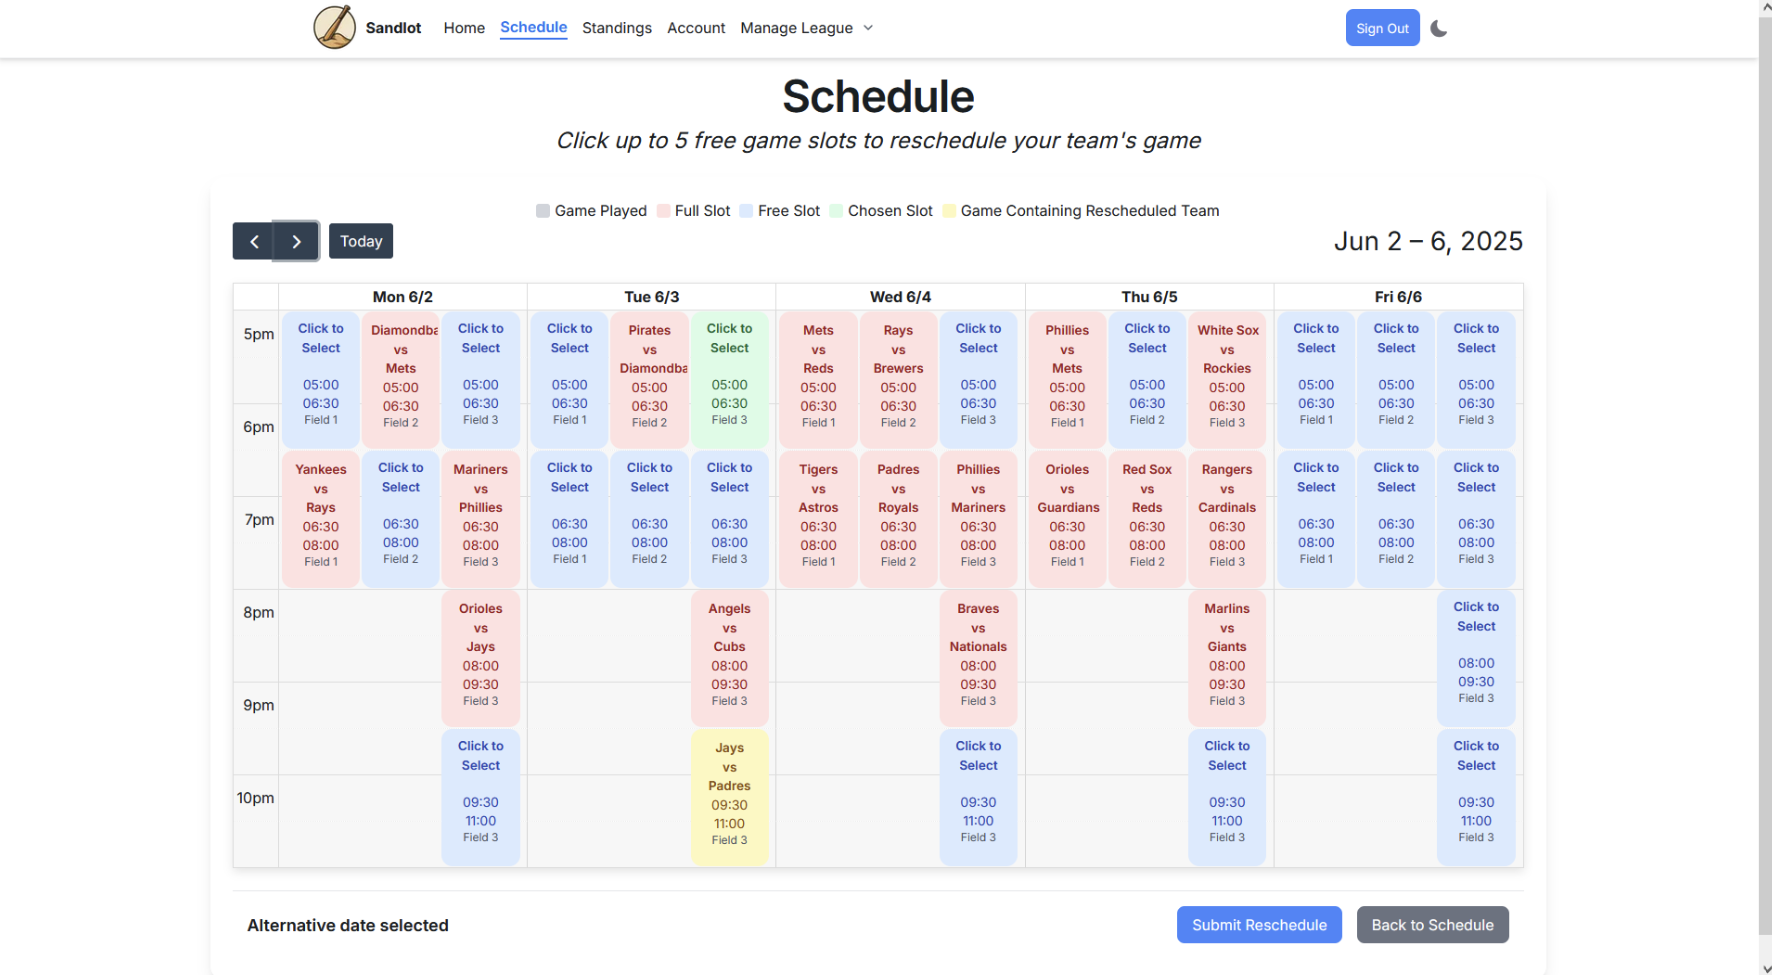
\includegraphics[scale=0.6]{rescheduling_improvement.png}
    \caption{Rescheduling Improvement}
    \label{rescheduling}
    \end{figure}
    
    The scheduling
    feature performed well in 43 out of 50 attempts, with occasional failures that
    resolved upon page reload, suggesting potential front-end improvements.

    Overall, the platform is functional and user-friendly but could benefit from
    refinements in security, error messaging, and performance optimization.
    The figures below showcase some of the data that was gathered from
    participants and used to improve the system's existing functions.

\section{Appendix}
    
    \begin{figure}[H]
    \centering
    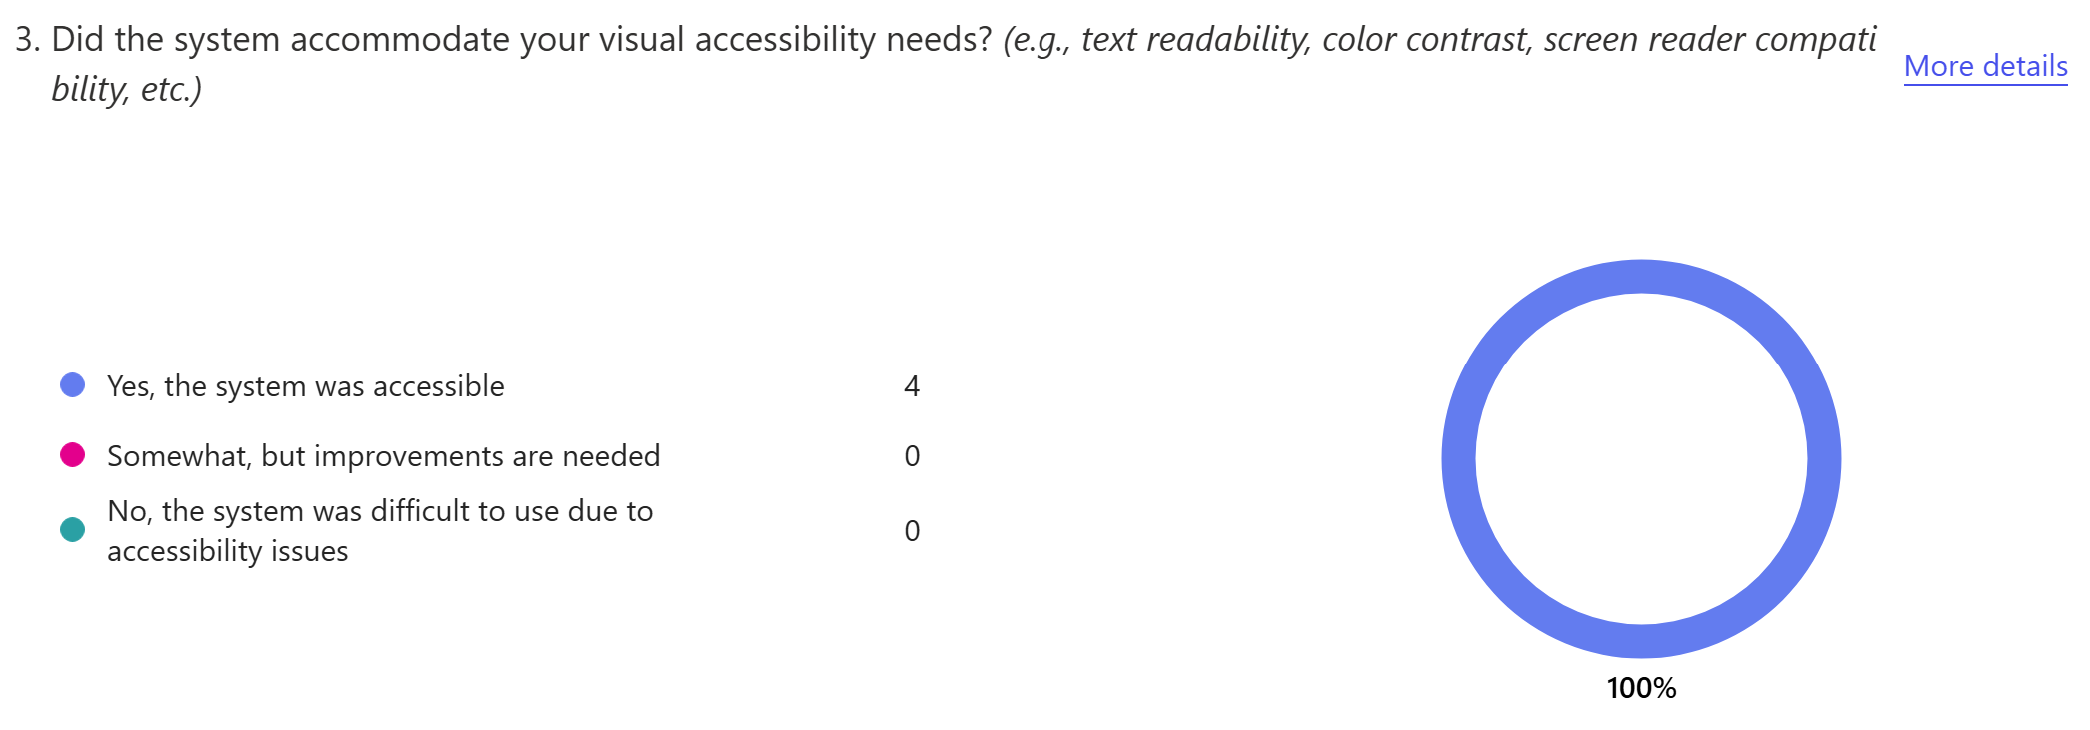
\includegraphics[scale=0.6]{survey_responses_visual.png}
    \caption{Readability Response Metrics}
    \label{visual}
    \end{figure}
    
    \begin{figure}[H]
    \centering
    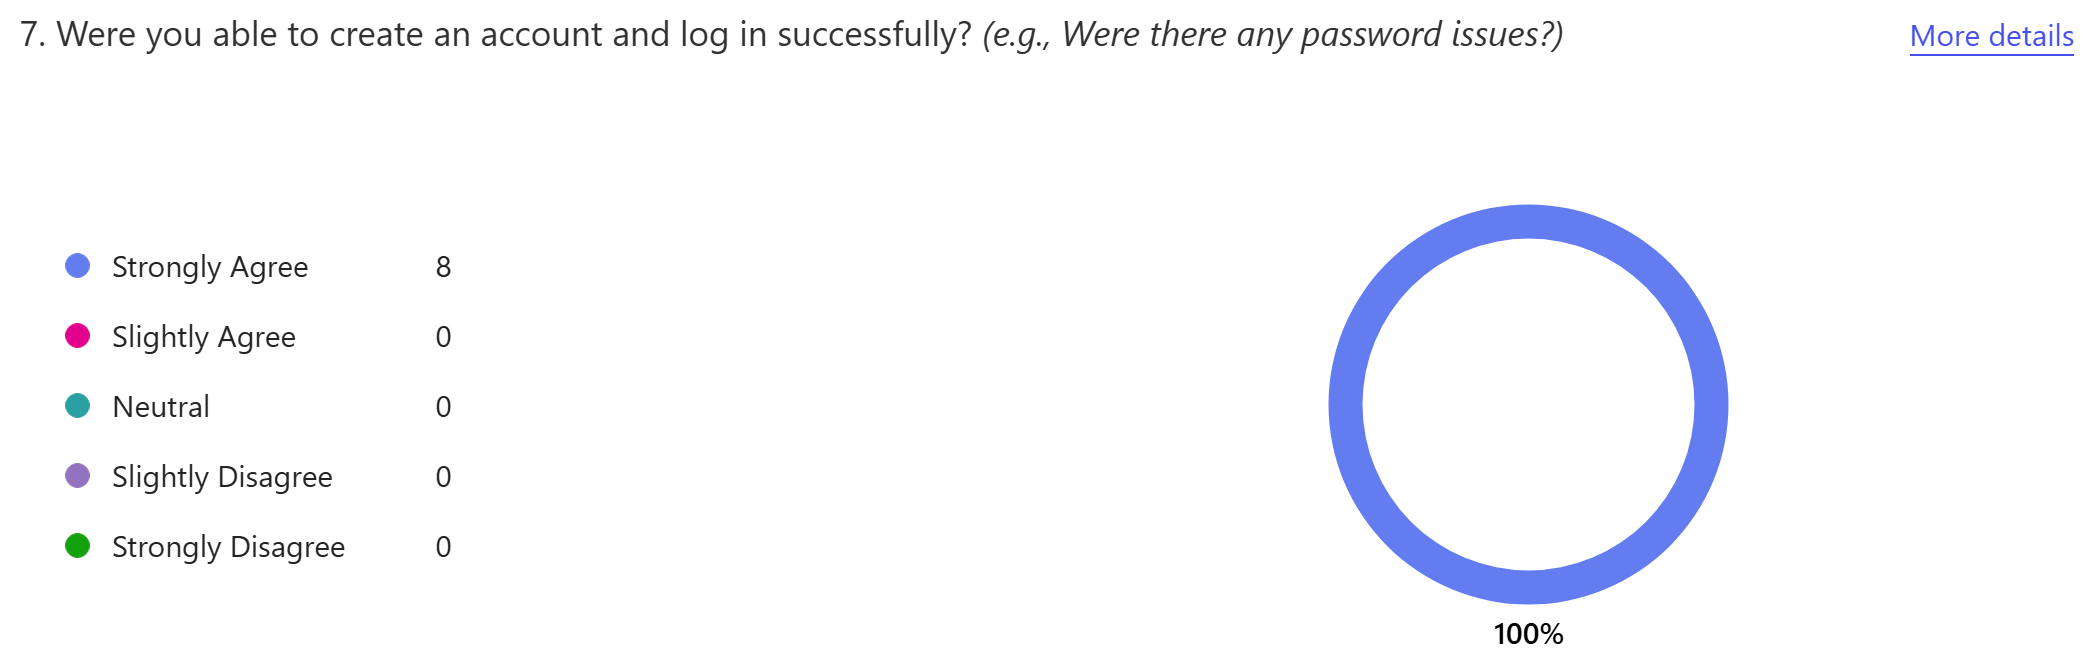
\includegraphics[scale=0.6]{survey_responses_register_signin.png}
    \caption{Registration/Login Response Metrics}
    \label{account}
    \end{figure}

    \begin{figure}[H]
    \centering
    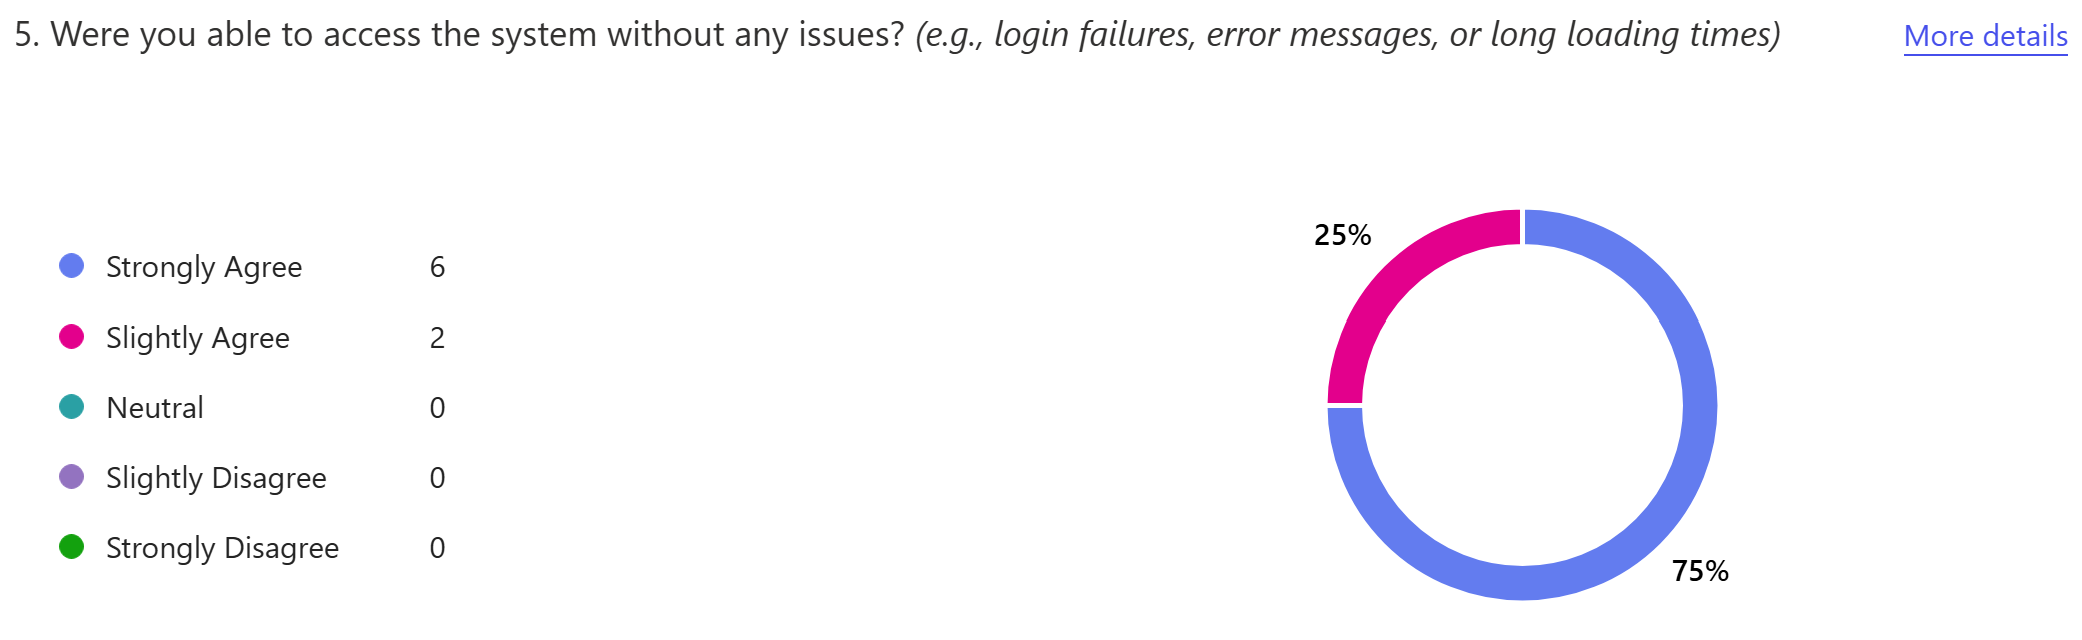
\includegraphics[scale=0.6]{survey_responses_access.png}
    \caption{General Access Response Metrics}
    \label{access}
    \end{figure}
    
    \begin{figure}[H]
    \centering
    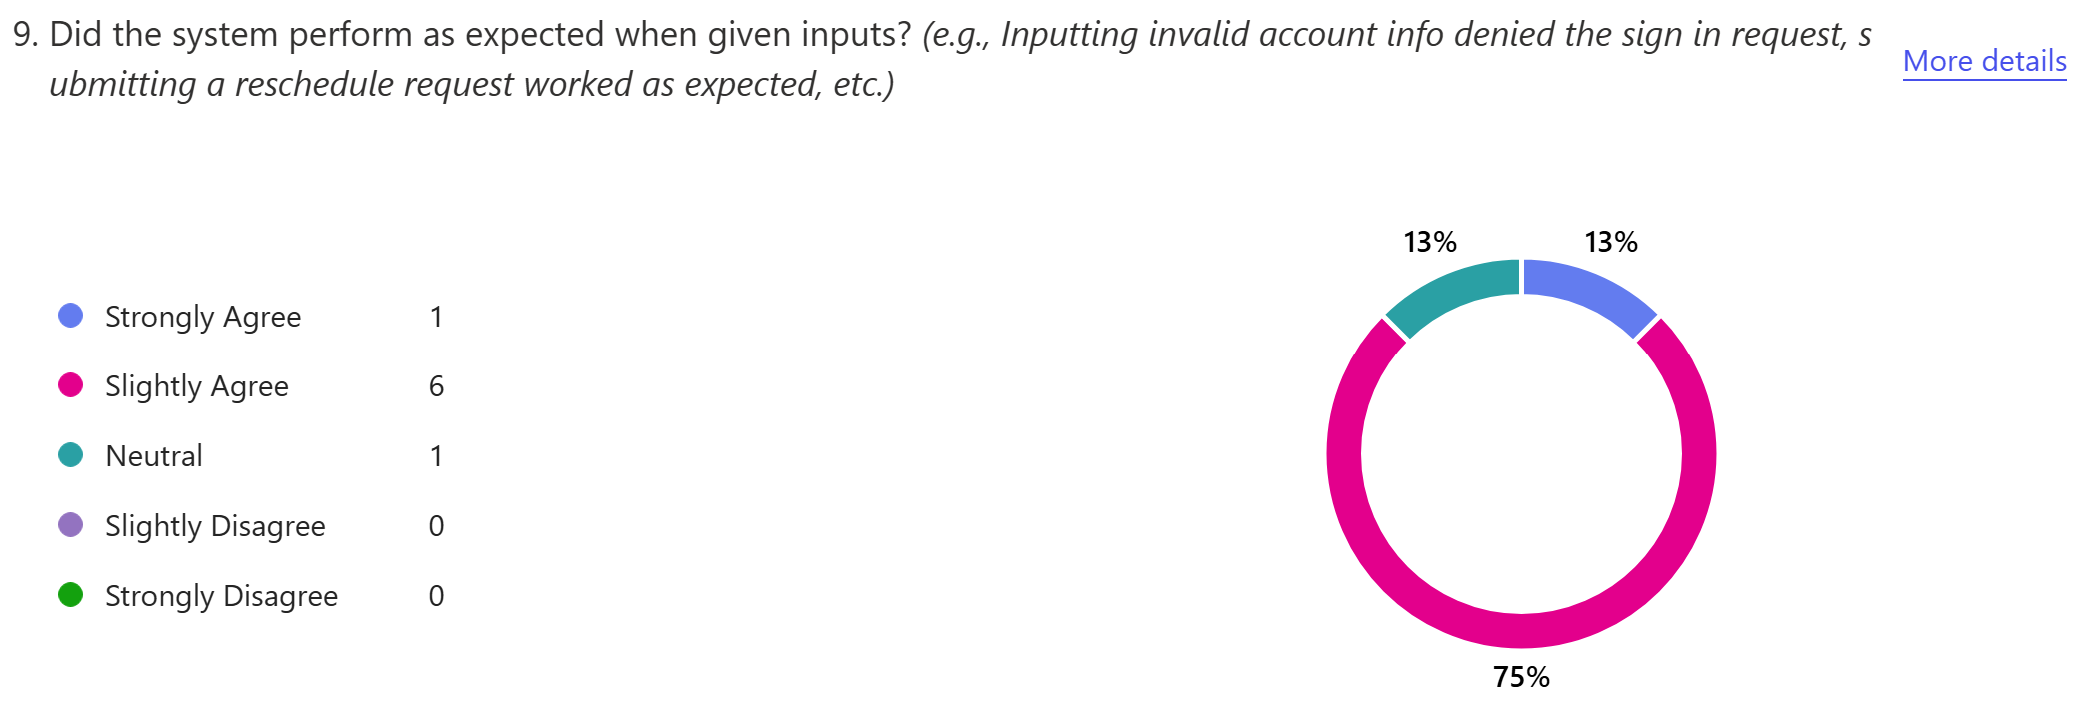
\includegraphics[scale=0.6]{survey_responses_validate_inputs.png}
    \caption{Request Validation Response Metrics}
    \label{validate}
    \end{figure}

    \begin{figure}[H]
    \centering
    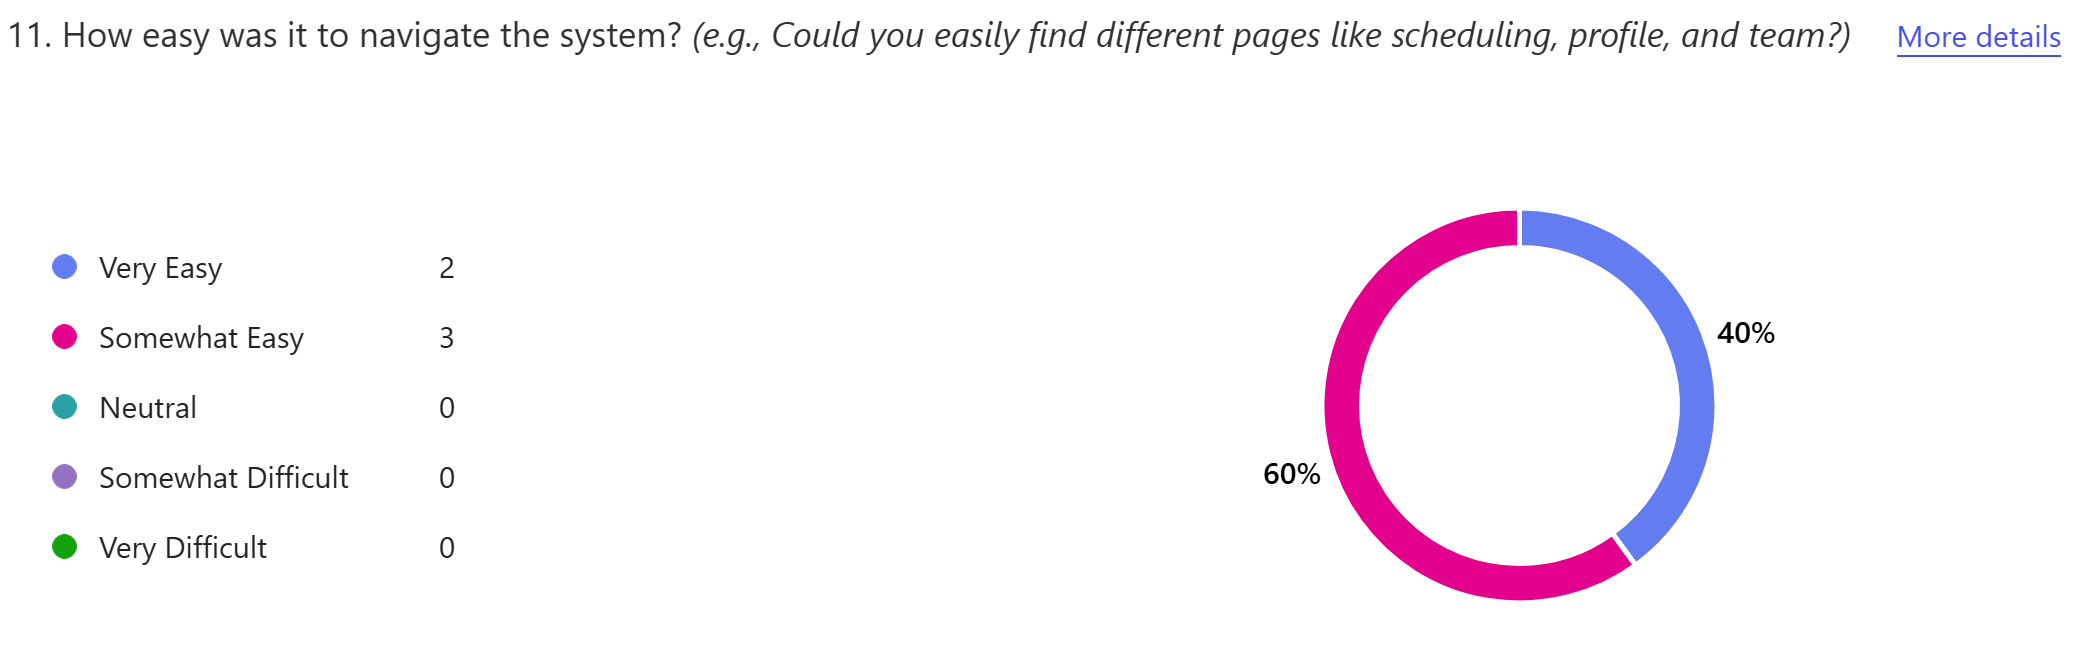
\includegraphics[scale=0.6]{survey_responses_navigation.png}
    \caption{Navigation Response Metrics}
    \label{nav}
    \end{figure}

\end{document}